\documentclass{mcmthesis}
\mcmsetup{CTeX = true,
	tcn = 0000,
	problem = A,
	sheet = true,
	titleinsheet = true,
	keywordsinsheet = true,
	titlepage = true,
	abstract = true
}

% Fakesection Customize
\usepackage{csvsimple}
\usepackage{exercise}
\usepackage{tasks}
\renewcommand{\ExerciseName}{Question}
\renewcommand{\AnswerName}{Answer}
\renewcommand{\listexercisename}{List of Questions}
\usepackage{subcaption}
\hypersetup{
	colorlinks = true,
	linkcolor = gray!75!black,
	citecolor = gray!75!black,
	backref = page
}
\usepackage[
	square, comma, numbers, super, sort&compress, longnamesfirst, sectionbib,
	nonamebreak
]{natbib}
\usepackage{boxie}

\begin{document}

% Fakesection Titlepage

\begin{abstract}

	To solve this problem, we use the method of principal component analysis
	to analyze the time series. We take two factors in consideration: the
	number of SCI, EI and papers respectively, and the number of students,
	average score, number of students under the guidance of tutors; Finally,
	we get the related formulas and give the reliable prediction results.
	The conclusion of sensitivity test shows that the model is robust.

	\begin{keywords}
		PCA; Factor Analysis; Time Series ;
	\end{keywords}

\end{abstract}

\title{\textbf{Research on graduate early warning model}}
\maketitle

% Fakesection Contents

\tableofcontents

\newpage

\listoffigures
\listoftables
\listofexercises

\newpage

\section{Introduction}%
\label{sec:Introduction}

In today's world, the graduation problem of college students has become
increasingly serious. Many college students can't even finish their studies on
time, so they are eliminated. Therefore, it is of great significance to analyze
the graduation problems of college students.

Doctoral education is the highest level of graduate education. The level of
doctoral education not only reflects the level of national higher education, but
also reflects the level of national scientific research. In recent years, with
the rapid growth of doctoral students, the phenomenon that doctoral students can
not graduate on time is becoming more and more common, which has become the
focus of social attention and discussion in recent years. However, there are
various and complex reasons that affect the overdue graduation of doctoral
students. How to find out the key factors and the degree of influence that
affect the overdue graduation of doctoral students, so as to take effective
measures to strengthen management, cultivate doctoral students in line with
social needs within the specified time, minimize the number of overdue graduates
and timely transport high-level talents for the country, is what this study
should explore . It is the core theme of this study. According to the doctoral
data of a university as the supporting data of the whole research, we find out
the key factors influencing the doctoral delay through factor analysis, and on
this basis, we calculate the score coefficient of the factors, and take the
graduation indicators of the University as the required data, which are not
mentioned in all policies. We use the standard value for processing, and succeed
This paper proposes a model of overdue warning. According to the theory of
sampling, the number of graduates who may graduate in the next year and the
number of those who may delay their graduation can be predicted from the sample
to the whole.
\cite{Wang2013Research,Yan2009Research,Wang2009Research}

\section{Analysis of the Problem}%
\label{sec:Analysis of the Problem}

Colleges and research institutes in China recruit a large number of graduate
students every year. After several years of study, these graduate students
should graduate from their own colleges and research institutes. At present, the
graduate situation of each unit is not optimistic, and the number of graduate
students who can not graduate smoothly for various reasons is increasing year by
year, which gradually attracted the attention of relevant units and the Ministry
of education.

Please establish the relevant mathematical model according to the study
conditions of graduate students (Master's degree and Doctor's degree) of Nanjing
University of Science and Technology (NJUST) over the years, so as to provide
decision-making reference for graduate school to send graduation warning to some
graduate students who may not graduate successfully in normal time. The specific
problems are as follows:

\begin{Exercise}

	Establish a mathematical model, and give the main factors and
	proportion that affect graduate students to graduate smoothly in
	normal time.

\end{Exercise}

\begin{Exercise}

	Establish a mathematical model, give an early warning one year in
	advance, and give a suggestion to extend the study (extend the
	time) and an evaluation standard to terminate the study.

\end{Exercise}

\begin{Exercise}

	Establish a mathematical model to predict the graduate students
	who will graduate smoothly and need to extend their studies
	(including the extension of time) in 2020 in Nanjing University
	of Science and Technology.

\end{Exercise}

\section{Calculating and Simplifying the Model}%
\label{sec:Calculating and Simplifying the Model}

Factor analysis is a statistical method used to describe variability among
observed, correlated variables in terms of a potentially lower number of
unobserved variables called factors. For example, it is possible that variations
in six observed variables mainly reflect the variations in two unobserved
(underlying) variables. Factor analysis searches for such joint variations in
response to unobserved latent variables. The observed variables are modelled as
linear combinations of the potential factors, plus "error" terms. Factor
analysis aims to find independent latent variables.

The theory behind factor analytic methods is that the information gained about
the interdependencies between observed variables can be used later to reduce the
set of variables in a dataset. Factor analysis is commonly used in biology,
psychometrics, personality theories, marketing, product management, operations
research, and finance. It may help to deal with data sets where there are large
numbers of observed variables that are thought to reflect a smaller number of
underlying/latent variables. It is one of the most commonly used
inter-dependency techniques and is used when the relevant set of variables shows
a systematic inter-dependence and the objective is to find out the latent
factors that create a commonality.

Factor analysis is related to principal component analysis (PCA), but the two
are not identical. There has been significant controversy in the field over
differences between the two techniques (see section on exploratory factor
analysis versus principal components analysis below). PCA can be considered as a
more basic version of exploratory factor analysis (EFA) that was developed in
the early days prior to the advent of high-speed computers. Both PCA and factor
analysis aim to reduce the dimensionality of a set of data, but the approaches
taken to do so are different for the two techniques. Factor analysis is clearly
designed with the objective to identify certain unobservable factors from the
observed variables, where as PCA does not directly address this objective; at
best, PCA provides an approximation to the required factors. From the point of
view of exploratory analysis, the eigenvalues of PCA are inflated component
loadings, i.e., contaminated with error variance.

We take two factors in consideration:

\begin{enumerate}

	\item SCI, EI, papers;

	\item Undergraduate school level, average score, number of students
		under the guidance of tutors;

\end{enumerate}

Factors that influence whether a doctoral student can graduate are divided into
scientific research factors and platform factors. Factor analysis was performed
on the relevant data obtained. Factor analysis is based on correlations between
variables, and based on these correlations, variables are combined to form the
smallest “factor”, representing the total change in the variables, simplifying
the variables, Clarify why. Scientific research factors are clearly divided into
the number of SCI publications, the number of EI publications, and the number of
general articles published. The platform elements are the undergraduate level,
the average grade of the course, the instructor-led students Is divided into a
number of. The calculation method for the doctoral degree evaluation index is
based on the establishment of the above evaluation index set matrix and the
standardization of data, and the correlation coefficient matrix R is calculated
according to the following formula.

\begin{align}
	(r_{jk})_{m \times m} = \frac{1}{N}\sum_{i = 1}^N Y_{ij}Y_{ik}
	(j,k = 1, 2, ..., m)
\end{align}

The results of the factor analysis are as table \ref{tab:Result}.

\begin{table}[htbp]
	\centering
	\caption{Result}
	\label{tab:Result}
	\csvautobooktabular{tab/result.csv}
\end{table}

The results of factor analysis indicate that among the factors in scientific
research, the SCI factor and EI factor are the main factors. At the platform
factor, students' courses are divided into key factors. The total number of
published articles, fresh graduates, and subject opening hours has a secondary
effect on whether a doctoral student can graduate.

At the same time, we also obtained the following results: First, the number of
doctoral students who published the SCI and EI papers had a significant impact
on their ability to end time, while overall the number of doctoral students who
publish ordinary papers has little effect on their ability to finish time. .
Second, the level of students in undergraduate schools, the average course
scores and the number of students their teachers teach have a significant impact
on their ability to graduate, but opening hours. on the topic and whether new
doctoral students are having less impact.

The SCI factor and the EI factor, the level of primary school for doctoral
students, the average number of study points and the number of students
supervised by the tutor have a greater influence on the successful completion of
doctoral students. The influence of time and doctoral degree on new students is
relatively small. It illustrates the need to offer courses at the doctoral
stage. The more scientific papers published by doctoral students during their
studies, the more they can complete their studies in good time, which also
confirms the universities' requirements for the publication of scientific
research results by doctoral students. The smaller the number of students led by
the tutor, the more an individual student can be advised, and the more likely it
is that the tutor will offer inexpensive instructions and various practical aids
for the completion of the doctoral students.

\section{The Model Results}%
\label{sec:The Model Results}

\begin{figure}[htbp]
	\centering
	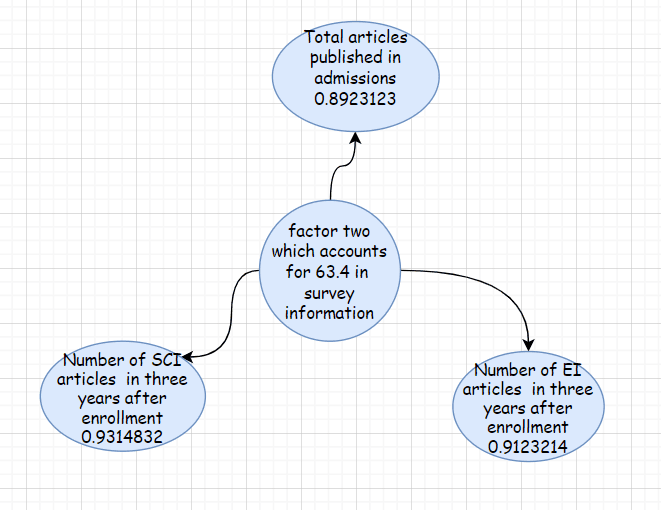
\includegraphics[width = 0.8\linewidth]{1.jpg}
	\caption{Factor1}
	\label{fig:Factor1}
\end{figure}

After choosing two main factors, the larger the contribution rate, the more able
to reflect the effect of the main factor on the completion time. For each main
factor, the closer the internal value of the main factor load matrix is to 1,
the greater the impact of the corresponding index on delat graduation, The two
main factors and related indicators are shown in Figures 1,2,and 3 as follows:
From the main factor that accounts for the largest contribution rate in Figure
1, it can be seen that the three factors that affect the delay graduation time
are total SCI published in three years、total articles published in admission
and total EI publshed in three years, so we consider the main factor as a
scientific research factor. This is also consistent with the current policy of
various universities, that is, publishing several papers that meet the grade,
such as professional journals such as SCI and EI. Of course, we can also see
that the scores of factors after the rotation factor are not as influential as
those of ordinary journals Impact factor journals are more influential.

\begin{figure}[htbp]
	\centering
	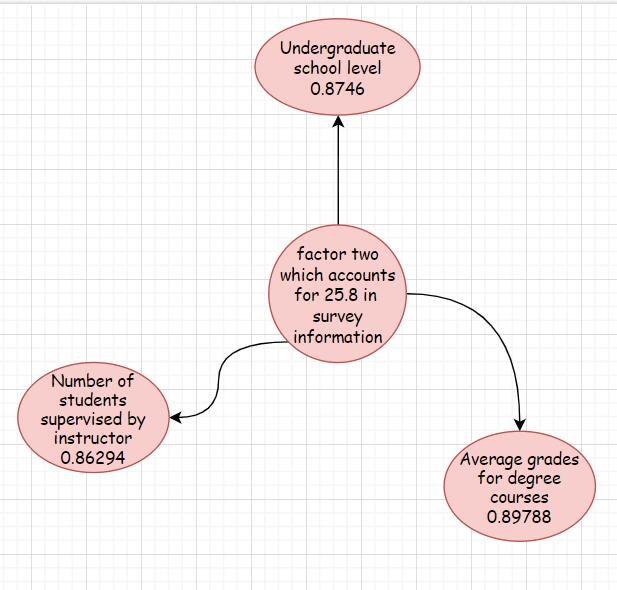
\includegraphics[width = 0.8\linewidth]{2.jpg}
	\caption{Factor2}
	\label{fig:Factor2}
\end{figure}

As can be seen from the main factor 2 which accounts for 25.8\% of the
contribution rate in Figure2,the three factors affecting delay graduation time.
Main factor two is named platform factor by us, which includes the grade of
undergraduate school, the number of students under the guidance of tutors, and
the weighted academic performance of normal courses. The main factor two
reflects the impact of a good platform on the delay time. If the undergraduate
receives more systematic discipline training, the higher the tutor's teaching
level, coupled with the individual efforts of students, will greatly reduce the
possibility of delay. Especially for personal factors, we can see that the
rotated factors are very close to 0.9.

\begin{figure}[htbp]
	\centering
	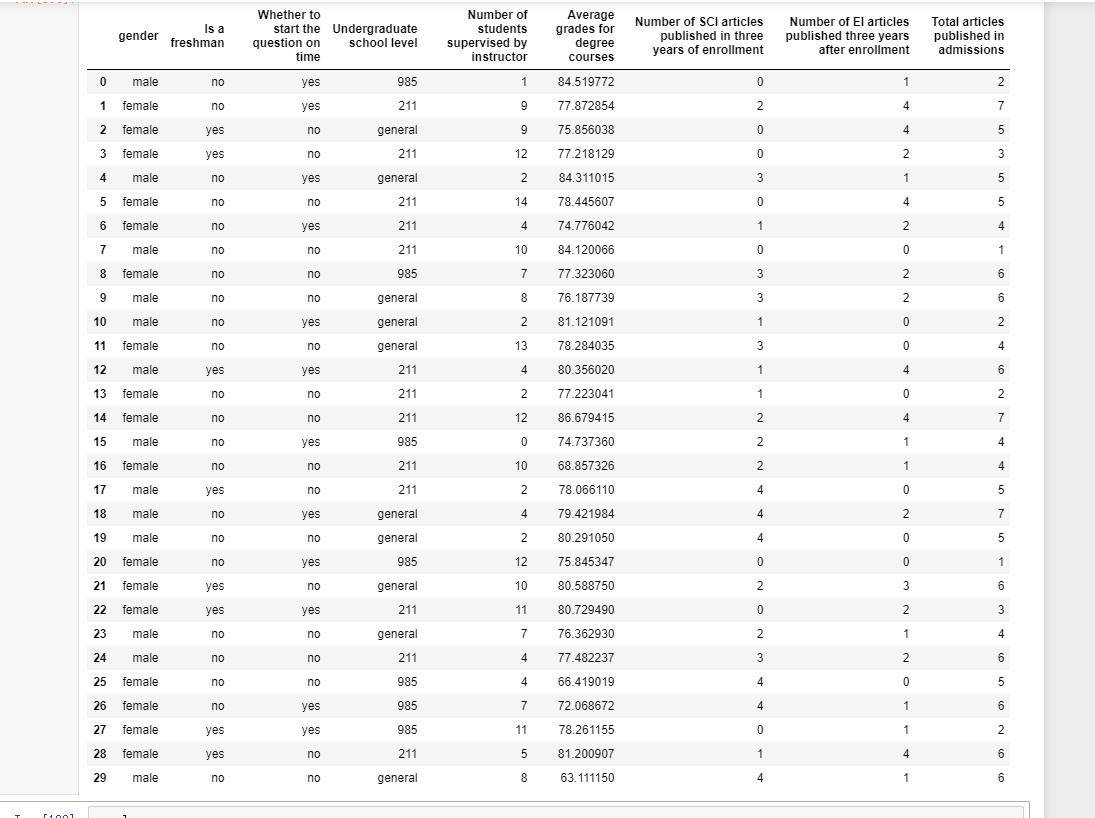
\includegraphics[width = 0.8\linewidth]{tab1.jpg}
	\caption{Result1}
	\label{fig:Result1}
\end{figure}

Figure \ref{fig:Result1} show that the data source is based on a questionnaire
survey from the academic research center of a university. Because there are a
lot of data with missing values, it will affect the distribution of the overall
variable. So in this process we filter out some missing values and follow After
processing the data, a 238 rows and 10 columns DataFrame table was obtained. The
table serves as a quantitative criterion for evaluating a doctoral student,
including whether it is gender, Is a freshman, Whether to start the question on
time, Undergraduate school level, Number of students supervised by instructor,
Average grades for degree courses, Number of SCI articles published in three
years of enrollment, Number of SCI articles published within 4 years of
enrollment, Number of EI articles published three years after enrollment, Total
articles published in admissions. In order to analyze the distribution of data,
we calculate some basic characteristics of the data set, including min, max, std
and other attributes.

\begin{figure}[htbp]
	\centering
	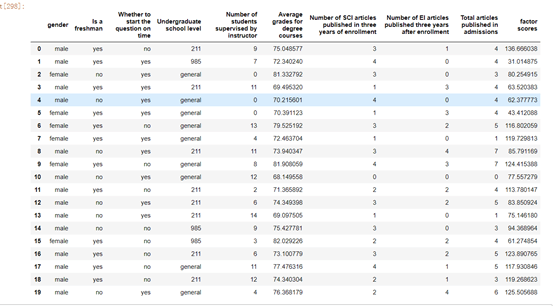
\includegraphics[width = 0.8\linewidth]{tab2.jpg}
	\caption{Result2}
	\label{fig:Result2}
\end{figure}

As figure \ref{fig:Result2}, we use the relationship between the factor
scores to successfully calculate the factor scores of the Ph.D. in three years,
and obtain the minimum factor score corresponding to the actual extension, and
use this value to determine whether the doctoral students can graduate normally.
In this case, because the data we collected are all data one year before
graduation, the implementation of the model may change due to changes in the
specific policies of the school, so this model has limitations, but it is
sufficient to roughly judge whether it is a certain period of time. The result
of being able to graduate on time.

According to statistical analysis, we can conclude that when the factor score is
greater than 99.017585, we must graduate on time. When the factor score is less
than 78.173158, the possibility of postponing graduation will greatly increase.
When in between, it should be noted that the possibility of delay will greatly
increase.

\begin{figure}[htbp]
	\centering
	\begin{subfigure}[htbp]{.45\linewidth}
		\centering
		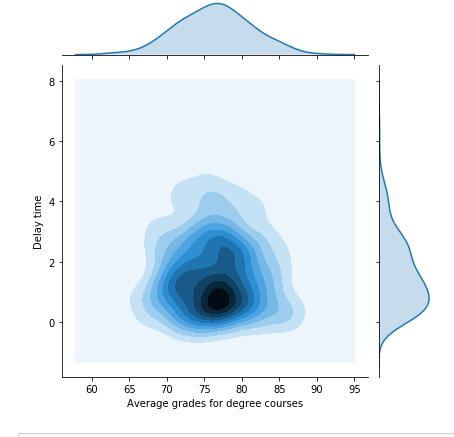
\includegraphics[width = 0.8\linewidth]{density.jpg}
		\caption{Delay Time1}
		\label{fig:Delay Time1}
	\end{subfigure}
	\quad
	\begin{subfigure}[htbp]{.45\linewidth}
		\centering
		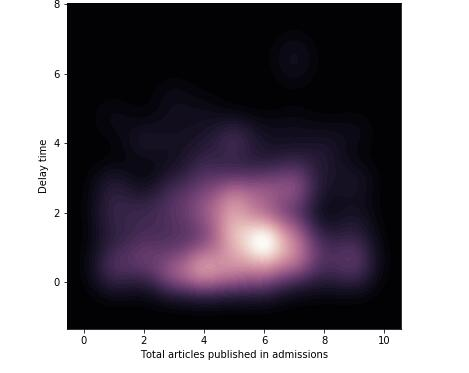
\includegraphics[width = 0.8\linewidth]{heat.jpg}
		\caption{Delay Time2}
		\label{fig:Delay Time2}
	\end{subfigure}
	\caption{Delay Time}
	\label{fig:Delay Time}
\end{figure}

We can see from the data set that there are three types of classification
attributes, namely gender, the level of the undergraduate school, whether it is
a freshman, and whether the question is opened on time. According to my own
understanding of the whole problem, so I made a corresponding pivot table to
provide more relevant information about the data. We can also provide more input
data sources for our factor analysis based on this pivot table, and more Data
combination form.

\section{Evaluate of the Mode}%
\label{sec:Evaluate of the Mode}

\subsection{Strengths}%
\label{sub:Strengths}

Factor analysis is an extension of multiple regression analysis, including some
modifications that make the approach less likely to be influenced by the
personal biases of the researcher, and less dependent on the assumption of
independence among variables. Technical explanations of factor analysis at
various levels of difficulty can be found in the books by Norušis (1994), Kline
(1994), Yotopoulos and Nugent (1976), and Mulaik (1974).

Ideally, in multiple regression analysis, one would observe a dependent variable
on the left hand side of an equation that is “explained” by a set of independent
variables on the right hand side. The problem, however, is that the connecting
link between dependent and independent variables needs a strong theoretical
basis. Furthermore, many of the so called “independent” variables may not really
be independent at all, but rather change or move together in response to some
other unknown variables or “factors.” Hence the researcher usually encounters
criticism of both the proposed theoretical framework and the method of
untangling the mutual dependence among the presumably independent variables.

In contrast, factor analysis is used to determine the underlying determinants of
many variables, without the need to postulate causality. This is especially
useful because economic and social indicators are closely intertwined, making it
nearly impossible to find a set of economic and social variables that are not
correlated in some way. This interdependence makes normal regression analysis
problematic but, surprisingly, does not adversely affect factor analysis.

Factor analysis, then, is a formal mathematical procedure that estimates the
unobserved independent factors (or components) that characterize the various
socalled independent variables. Because they can be constructed to be
independent, the factor estimates (called factor scores) can be used in
regression analysis to find the correlation between the factors and the
dependent variable. The dependent variable may or may not be incorporated
directly into the procedure that estimates the independent factors. If one is
looking to estimate a missing observation for a dependent variable, such as per
capita GDP for a particular country (as is the goal of this study) then this
variable is not made part of the procedure.

The mathematical procedure is less likely to be influenced by the personal
biases of the researcher because he or she is supposed to include as many
variables as possible, allowing it to dictate how the variables are grouped
together into factors. It is also usually found that a much smaller number of
factors than variables is able to explain most of the variance of any of the
variables included in the procedure, or later used as a dependent variable.

\subsection{Weaknesses}%
\label{sub:Weaknesses}

There are still many shortcomings or limitations in research.

First, there are some shortcomings in model construction and support for
variables in the study.  Potential variables are the academic basis of PhD
students and their research potential. Their effective measurement is an
important part of the analysis of the reasons for the delayed completion of
doctoral students. Due to the lack of necessary information, there is no
research on the possible impact of this factor on graduation. Make direct
estimates. In the study, although the number of meetings with the mentor were
used as the time of advice, and various academic titles were used as indicators
to measure the mentor's professional level, there was some rationality, but the
service was simple and deviations may occur. Factors such as doctoral student
fertility status, thesis opening time, mentor size, mentor status, and the work
environment can also affect postgraduate studies. Due to data limitations, the
study did not analyze these variables.

Secondly, the training of doctoral students under the tutor system has
distinctive individual characteristics, and model-based interpretation is
generalized. The mechanism of influence of different factors is still an issue
that needs to be further explored in future research. Among the reasons for the
delay, which are caused by factors in the education system, which are caused by
other external factors, and the relationship between different factors, these
are all factors that should be paid attention to when discussing the
relationship between the factors and the doctoral students. Third, the research
sample has limitations. The conclusions of the research are based on data from
only one university. The relevant conclusions only partially verify some factors
that affect the postgraduate completion of the doctoral degree. These
conclusions are applicable to other doctoral education units. Sex has yet to be
tested.

% Fakesection Reference

\newpage

\addcontentsline{toc}{section}{Reference}

\bibliographystyle{IEEEtran}
\bibliography{bib/main}

\begin{appendices}

	\section{Code}

	\langCVfile[python][lst:main.py][python]{main.py}{lst/main.py}

	\section{Data}

	\begin{table}[htbp]
		\centering
		\caption{Data}
		\label{tab:Data}
		\csvautobooktabular{tab/data.csv}
	\end{table}

\end{appendices}

\end{document}

